% example.tex
\documentclass[dvisvgm]{standalone}

\usepackage[usenames,dvipsnames]{xcolor}
\usepackage{tikz}
\usetikzlibrary {positioning,
                 shapes.geometric}

\tikzset{
         square/.style={regular polygon, regular polygon sides=4},
         myarrow/.style={-Stealth, line width=0.25mm},
}

\begin{document}
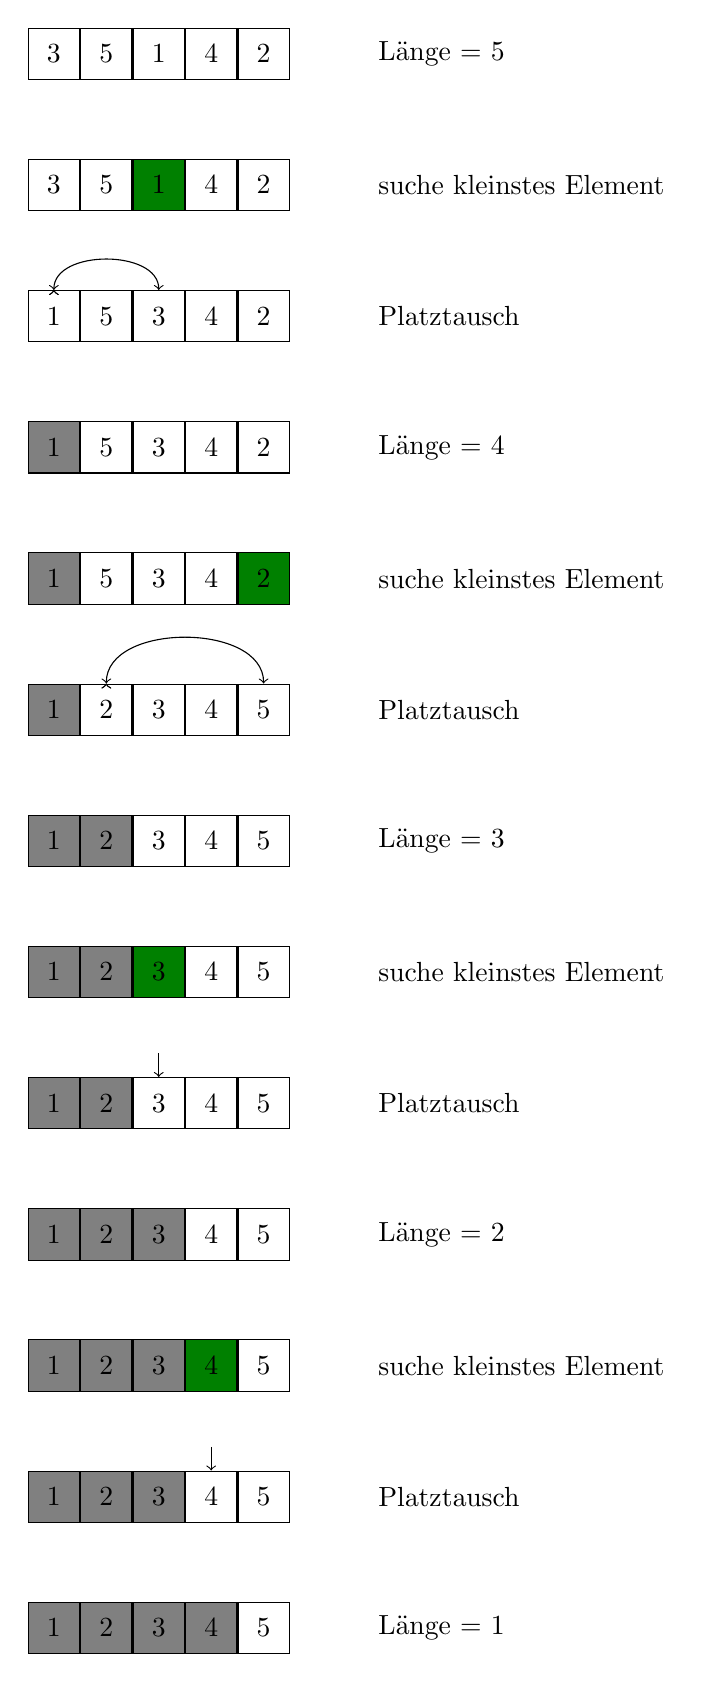
\begin{tikzpicture}
    % Grundmuster
    \node[draw, square] (a) {3}; 
    \node[draw, square, right=0cm of a] (b) {5};
    \node[draw, square, right=0cm of b] (c) {1};
    \node[draw, square, right=0cm of c] (d) {4};
    \node[draw, square, right=0cm of d] (e) {2};
    \node[right= of e] (e_text) {Länge = 5};

    % S1.1
    \node[draw, square, below = of a] (a11) {3}; 
    \node[draw, square, right=0cm of a11] (b11) {5};
    \node[fill=Green,
          draw, square, right=0cm of b11] (c11) {1};
    \node[draw, square, right=0cm of c11] (d11) {4};
    \node[draw, square, right=0cm of d11] (e11) {2};
    \node[right= of e11] (e11_text) {suche kleinstes Element};

    % S2.1
    \node[draw, square, below = of a11] (a21) {1}; 
    \node[draw, square, right=0cm of a21] (b21) {5};
    \node[draw, square, right=0cm of b21] (c21) {3};
    \node[draw, square, right=0cm of c21] (d21) {4};
    \node[draw, square, right=0cm of d21] (e21) {2};
    \node[right= of e21] (e21_text) {Platztausch};
    \draw[<->] (a21.north) edge [bend left = 90] (c21.north);


    % S3.1
    \node[fill=Gray,
          draw, square, below = of a21] (a31) {1}; 
    \node[draw, square, right=0cm of a31] (b31) {5};
    \node[draw, square, right=0cm of b31] (c31) {3};
    \node[draw, square, right=0cm of c31] (d31) {4};
    \node[draw, square, right=0cm of d31] (e31) {2};
    \node[right= of e31] (e21_text) {Länge = 4};


    % S1.2
    \node[fill=Gray,
          draw, square, below = of a31] (a12) {1}; 
    \node[draw, square, right=0cm of a12] (b12) {5};
    \node[draw, square, right=0cm of b12] (c12) {3};
    \node[draw, square, right=0cm of c12] (d12) {4};
    \node[fill=Green,
          draw, square, right=0cm of d12] (e12) {2};
    \node[right= of e12] (e21_text) {suche kleinstes Element};

    % S2.2
    \node[fill=Gray,
          draw, square, below = of a12] (a22) {1}; 
    \node[draw, square, right=0cm of a22] (b22) {2};
    \node[draw, square, right=0cm of b22] (c22) {3};
    \node[draw, square, right=0cm of c22] (d22) {4};
    \node[draw, square, right=0cm of d22] (e22) {5};
    \node[right= of e22] (e21_text) {Platztausch};
    \draw[<->] (b22.north) edge [bend left = 90] (e22.north);

    % S3.2
    \node[fill=Gray,
          draw, square, below = of a22] (a32) {1}; 
    \node[fill=Gray,
          draw, square, right=0cm of a32] (b32) {2};
    \node[draw, square, right=0cm of b32] (c32) {3};
    \node[draw, square, right=0cm of c32] (d32) {4};
    \node[draw, square, right=0cm of d32] (e32) {5};
    \node[right= of e32] (e21_text) {Länge = 3};

    % S1.3
    \node[fill=Gray,
          draw, square, below = of a32] (a13) {1}; 
    \node[fill=Gray,
          draw, square, right=0cm of a13] (b13) {2};
    \node[fill=Green,
          draw, square, right=0cm of b13] (c13) {3};
    \node[draw, square, right=0cm of c13] (d13) {4};
    \node[draw, square, right=0cm of d13] (e13) {5};
    \node[right= of e13] (e21_text) {suche kleinstes Element};

    % S2.3
    \node[fill=Gray,
          draw, square, below = of a13] (a23) {1}; 
    \node[fill=Gray,
          draw, square, right=0cm of a23] (b23) {2};
    \node[draw, square, right=0cm of b23] (c23) {3};
    \node[draw, square, right=0cm of c23] (d23) {4};
    \node[draw, square, right=0cm of d23] (e23) {5};
    \node[right= of e23] (e21_text) {Platztausch};
    \node[above=0.3cm of c23] (c23h) {};
    \draw[->] (c23h) edge (c23.north);

    % S3.3
    \node[fill=Gray,
          draw, square, below = of a23] (a33) {1}; 
    \node[fill=Gray,
          draw, square, right=0cm of a33] (b33) {2};
    \node[fill=Gray,
          draw, square, right=0cm of b33] (c33) {3};
    \node[draw, square, right=0cm of c33] (d33) {4};
    \node[draw, square, right=0cm of d33] (e33) {5};
    \node[right= of e33] (e21_text) {Länge = 2};

    % S1.4
    \node[fill=Gray,
          draw, square, below = of a33] (a14) {1}; 
    \node[fill=Gray,
          draw, square, right=0cm of a14] (b14) {2};
    \node[fill=Gray,
          draw, square, right=0cm of b14] (c14) {3};
    \node[fill=Green,
          draw, square, right=0cm of c14] (d14) {4};
    \node[draw, square, right=0cm of d14] (e14) {5};
    \node[right= of e14] (e14_text) {suche kleinstes Element};

    % S2.4
    \node[fill=Gray,
          draw, square, below = of a14] (a24) {1}; 
    \node[fill=Gray,
          draw, square, right=0cm of a24] (b24) {2};
    \node[fill=Gray,
          draw, square, right=0cm of b24] (c24) {3};
    \node[draw, square, right=0cm of c24] (d24) {4};
    \node[draw, square, right=0cm of d24] (e24) {5};
    \node[right= of e24] (e24_text) {Platztausch};
    \node[above=0.3cm of d24] (d24h) {};
    \draw[->] (d24h) edge (d24.north);

    % S3.4
    \node[fill=Gray,
          draw, square, below = of a24] (a34) {1}; 
    \node[fill=Gray,
          draw, square, right=0cm of a34] (b34) {2};
    \node[fill=Gray,
          draw, square, right=0cm of b34] (c34) {3};
    \node[fill=Gray,
          draw, square, right=0cm of c34] (d34) {4};
    \node[draw, square, right=0cm of d34] (e34) {5};
    \node[right= of e34] (e21_text) {Länge = 1};
\end{tikzpicture}
\end{document}
